\documentclass[10pt,twocolumn]{article}
\usepackage[utf8]{inputenc}
\usepackage{graphicx}
\usepackage{amsmath}
\usepackage{amssymb}
\usepackage{hyperref}
\usepackage{geometry}
\usepackage{cite}
\usepackage{xcolor}

\geometry{margin=1in}

\title{Improving Model Inversion Attacks Using Additional Backbones}
\author{Christopher Roßbach \\ FAU-Erlangen-Nürnberg}
\date{\today}

\begin{document}

\maketitle
\begin{abstract}
    Model inversion attacks aim to infer sensitive information about input or training data from the outputs or representations of machine learning models.
    In this work we explore model inversion in the form of reconstructing images from their feature embeddings in a known latent space.
    We explore the effectiveness of optimization based methods in different latent spaces.
    Using the discovered findings, we propose a method that leverages the embeddings of multiple reconstruction candidates in foreign latent spaces to improve reconstruction quality.
\end{abstract}

\section{Introduction}
Model inversion attacks pose significant risks by reconstructing private information about either training data or model inputs.
This report investigates techniques that try to reconstruct the full model input from a latent representation.
We limit ourselves to the task of image reconstruction from feature embeddings given by a pretrained vision backbone.
We assume a white-box setting where the attacker has access to the model architecture and parameters as well as the feature embedding of the target image.

We aim to approximate the private image $x^*$ owned by the victim from its embedding $y^* = f(x^*)$ where $f$ is a pretrained known backbone network and $y^*$ is the embedding known to the attacker (either leaked or purposely shared).

\section{Related Work}
Brief overview of previous research on model inversion attacks and defense mechanisms.


\section{Methodology}
We try to reconstruct the private image from its embedding through an optimization process.
The problem of reconstructing the private image from its embedding is a strongly ill posed which forces us to incorporate additional constraints and priors to the optimization process.
The optimization problem can be formulated as
$$
\min_{\hat{x}} d_f(f(\hat{x}), y^*) + \mathcal{R}(\hat{x}),
$$
where $\mathcal{R}$ is a regularization term that encourages the reconstruction to be smooth and natural and is further described in Section~\ref{reg}.
$d_f$ is a distance function that is dependent on the used backbone $f$.
For a ResNet backbone we use the mean squared error (MSE) as the distance function while using a cosine based distance for a clip encoder.
\subsection{The Iterative Base Method}\label{base_method}
We employ an iterative optimization method to progressively refine the reconstruction.
We generally optimize in the image space while resorting to a lower dimensional image space at the beginning of the reconstruction.
Successive upscaling encourages the reconstruction of coarse structures before refining details.
We take the resolution steps used in~\cite{kazemiWhatWeLearn2024} and find adding another low resolution step of 32 to be beneficial, resulting in a scale sequence of $n\in\{32, 64, 128, 224\}$ where upscaling is performed at steps 400, 900 and 1800.

At each iteration, we update the reconstruction $x$ in the possibly smaller space $\mathbb{R}^{3\times n \times n}$ from which we retrieve the full size reconstruction proposal $\mathbb{R}^{3\times N \times N}\ni\hat{x} = S_N(x)$ by using a differentiable scaling function $S_k:\mathbb{R}^{3\times n \times n}\rightarrow\mathbb{R}^{3\times k \times k}$.
The next reconstruction $x$ is determined by
\begin{equation}\label{eq:update_rule}
x^{(t)} = S_{n_t}\left(x^{(t-1)} - \eta \dfrac{\nabla \mathcal{L}(x^{(t-1)}, y^*)}{\|\nabla \mathcal{L}(x^{(t-1)}, y^*)\|_2}\right),
\end{equation}
where $t$ denotes the iteration step, $n_t$ the resolution at step $t$, $\eta$ is the learning rate, and $\mathcal{L}$ the loss function.
This process is repeated for 3000 iterations after which no notable improvement was noticed in practice.
Normally we perform multiple reconstructions in parallel, because the result depends on the initialization $x^{(0)}$.
We denote such a set of equally constructed reconstructions as $X^{(t)} = \{x^{(t)}_0, x^{(t)}_1, \dots, x^{(t)}_{m-1}\}$ where $m$ is the number of parallel reconstructions.

For now, the loss function $\mathcal{L}$ is defined as
\begin{equation}\label{eq:loss_function_base}
\mathcal{L}(x, y^*) = \mathcal{L}_{f}(x, y^*) + \mathcal{R}(S_N(x)),
\end{equation}
with
\begin{equation}\label{eq:loss_function_f}
    \mathcal{L}_f(x, y^*) = d_{f}(f(A(S_N(x))), y^*),
\end{equation}
where $A$ is a randomized augmentation function as described in Section~\ref{augs}, and $d_f$ is a distance function that is dependent on the used backbone $f$ and $\mathcal{R}$ is a regularization term as described in Section~\ref{reg}.

\subsection{Augmentations}\label{augs}
As proposed in~\cite{ghiasiPlugInInversionModelAgnostic2021} we employ a set of differentiable augmentations to improve the robustness of the reconstruction.
We expect the embedding to be stable under (slight) scaling, rotation and translation.
We incorporate these augmentations into the optimization process as a prior by applying a (different) set of augmentations at each step of the optimization.
The transformation is thereby chosen randomly from $(\text{scale}, \text{rotate}, \text{translate}_h, \text{translate}_v) \in \lbrack 0.7, 1.5\rbrack\times \lbrack -30, 30\rbrack \times \lbrack -0.1, 0.1\rbrack \times \lbrack -0.1, 0.1\rbrack$.

\subsection{Regularization}\label{reg}
For regularization we use a term based on total variation as proposed in~\cite{mahendranUnderstandingDeepImage2015} with the adjustment of using a $L_1$ distance:
$$
\mathcal{R}(x) = g_{\alpha,\beta}\left(\dfrac{\mathcal{R}_{TV}(x)}{(n-1)^2}\right)
$$
with
$$
\mathcal{R}_{TV}(x) = \sum_{i,j} \left| x_{i,j} - x_{i + 1,j} \right| + \left| x_{i,j} - x_{i,j + 1} \right|.
$$
This term is used to penalize sharp edges in the reconstructed images.
Here $n$ refers to the width of the square image and $g_{\alpha,\beta}$ is a penalty function that balances the contribution of the total variation term and is defined as:
$$
g_{\alpha,\beta}(x) = \text{relu}(x - \alpha) + \beta\cdot\text{relu}(x - \alpha) ^ 2.
$$
This quadratic dead zone penalty function allows for punishment-free variation in the interval $\lbrack-\alpha,\alpha\rbrack$ and (for big enough $\beta$) limits the total variation to be close to $\alpha$.
The use of this penalty function makes sure, that the this regularization term does not loose importance when adding additional terms to the objective function of the optimization.
A parameter selection of $\alpha = 0.3$ and $\beta = 10$ was found to yield good results in practice.\footnote{We could pin this to the avg value of e.g. ImageNet Data.}

\subsection{Impact of Inverted Model}
The reconstruction method described in Section~\ref{base_method} yields visibly different results when using different backbones $f$.
It is to note, that the reconstruction for different backbones does not strictly yield better or worse reconstructions, but rather reconstruction with qualitatively different details.
This effect can be seen in figure~\ref{fig:resnet_vs_clip}.

For the picture of the safe, we note that the reconstruction on a ResNet backbone gives a picture containg structural properties of a safe, while the reconstruction on the clip embedding seems to reproduce the text contained in the lower right corner of original picture.
For the dog picture, the reconstruction based on the clip embedding yields a better representation of the dog's features compared to the ResNet based reconstruction, while the ResNet reconstruction contains patterns of the background.
In the reconstruction of the fish picture the ResNet based reconstruction focuses on the fish's shape and the hands while the clip based reconstruction reconstructs the face of the person holding the fish.

From this observation we conclude, that a improvement in reconstruction quality can be achieved by combining different backbones in the reconstruction process while maintaining the assumption to have access to a single embedding.
\begin{figure}[ht]
    \centering
    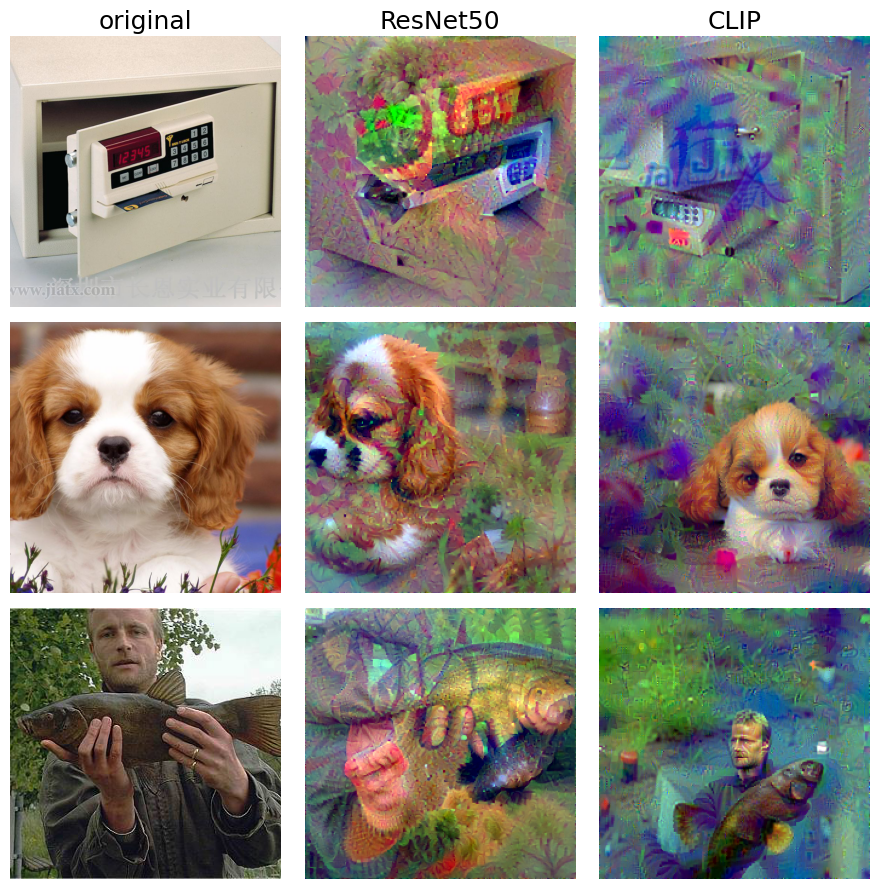
\includegraphics[width=\linewidth]{figures/resnet-vs-clip.png}
    \caption{
        Comparison of reconstructions on ResNet and CLIP backbones.
    }
    \label{fig:resnet_vs_clip}
\end{figure}

\subsection{Average of Foreign Embeddings}
Another important observation is that if we have two different backbones $f$ and $h$, a private image $x^*$ and a slightly modified version $x^*_p$ of the private image for which $f(x^*)\approx f(x^*_p)$ then we also observe $h(x^*)\approx h(x^*_p)$.
That is, if we modify the private image only slightly, the embeddings produced by different backbones remain consistent.
However, this behaviour does not apply to reconstructions: for a reconstruction $\hat x_f$ obtained by procedure described in~\ref{base_method} with respect to the backbone $f$ that suffices $f(\hat x_f)\approx f(x^*)$ we observe strong differences in the embedding under $h$, $d_h(h(\hat x_f),h(x^*)) \gg d_f(f(\hat x_f),f(x^*))\approx 0$.
The same is true for two different reconstructions $\hat x_{f,0}$ and $\hat x_{f,1}$: while $f(\hat x_{f,0})\approx f(\hat x_{f,1})$ we observe $h(\hat x_{f,0})\not\approx h(\hat x_{f,1})$.

Furthermore, if we have a set of reconstruction $X_f = \{\hat x_{f,0}, \hat x_{f,1}, \dots\}$ we observe that that the average embedding under $h$ of the reconstructions $X_f$ is closer to the embedding und $h$ of the private image then the average distance of the reconstructions: $$d_h\left(\overline{h(X_f)}, h(x^*)\right) < \overline{d_h(h(X_f), h(x^*))}.$$
We often observe the even stronger statement, that the averaged embedding is closer to the embedding of the private image then every single reconstruction: $$\forall\hat x_f \in X_f: d_h\left(\overline{h(X_f)}, h(x^*)\right) < d_h(h(\hat x_f), h(x^*)).$$
This effect can be seen in figure~\ref{fig:avg_distance_scatter}.
\begin{figure}[ht]
    \centering
    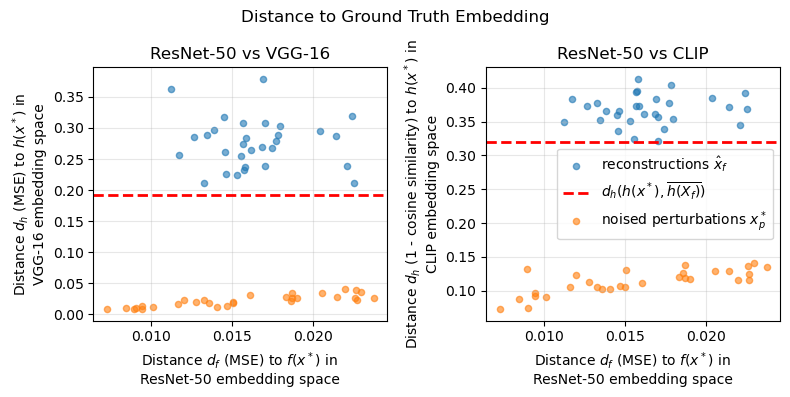
\includegraphics[width=\linewidth]{figures/avg-distance-scatter.png}
    \caption{
       Comparison of embedding distances for noised images, reconstructions and averaged reconstruction embeddings for $f$ being a ResNet backbone, and $h$ being a VGG backbone (left) and $h$ being a CLIP backbone (right).
    }
    \label{fig:avg_distance_scatter}
\end{figure}

That leads to the intuitive assumption the that embeddings under a foreign backbone $h$ scatter around the embedding of the private image $h(x^*)$ and do not deviate in a specific direction.
This idea is illustrated in figure~\ref{fig:avg_embedding_sketch}.
\begin{figure}[ht]
    \centering
    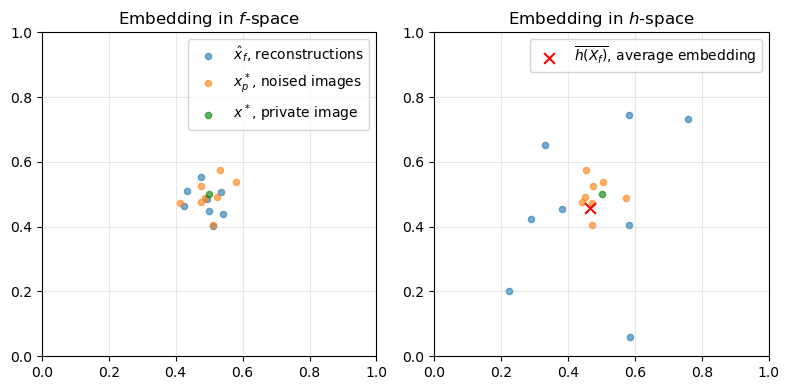
\includegraphics[width=\linewidth]{figures/avg-embedding-sketch.png}
    \caption{
       Illustration of the imagined scattering behavior of embeddings under a backbone used for reconstruction $f$ (left) and a foreign backbone $h$ (right).
       The average embedding in the foreign space is closer to the embedding of the private image than the embeddings of the reconstructions.
    }
    \label{fig:avg_embedding_sketch}
\end{figure}

\subsection{Combining Multiple Backbones}\label{combining_backbones}
To potentially make use of this we explored multiple methods to incorporate the average in the foreign embedding space during the reconstruction process.

Since most of the used networks apply a ReLu activation as their last non-linearity, simply calculating the arithmetic average in each coordinate leads to a huge shift in the shape of the distribution of embeddings.
To reduce that shift, we can perform the averaging in the latent space before applying the last ReLu activation.
The effect of this can bee seen in figure~\ref{fig:relu_norelu_distribution_shift}.
We perform the experiments on both, the truncated and the original backbones.

\begin{figure}[ht]
    \centering
    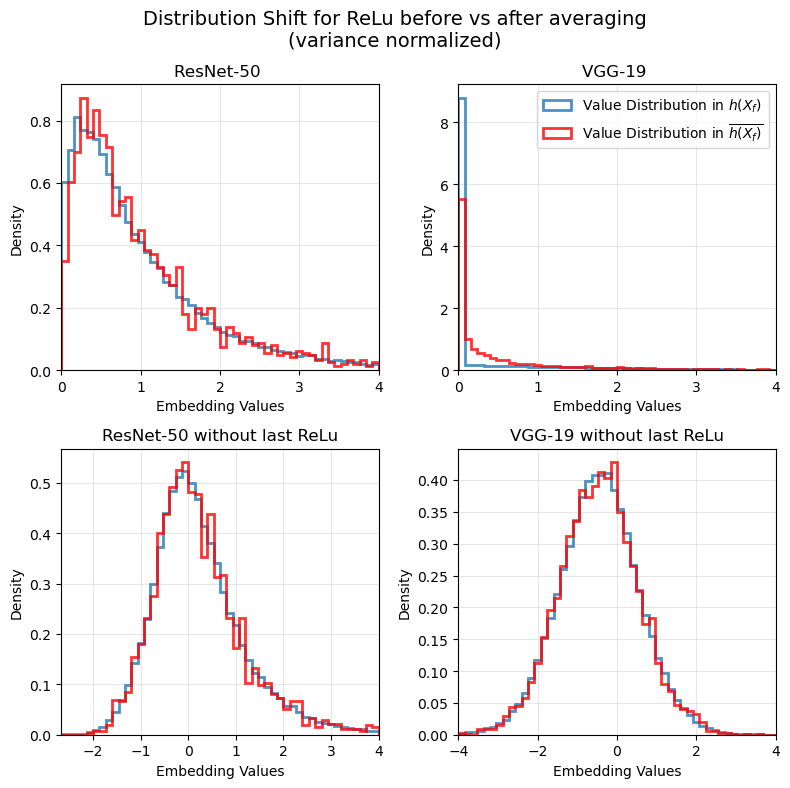
\includegraphics[width=\linewidth]{figures/relu-norelu-distribution-shift.png}
    \caption{
       Distribution of embeddings in different backbones.
       Top: Value distribution under original backbone.
       Bottom: Value distribution under modified backbone with the last ReLu removed.
    }
    \label{fig:relu_norelu_distribution_shift}
\end{figure}

We incorporate the average embedding in a foreign space by extending loss function from equation~\ref{eq:loss_function_base}:
\begin{equation}\label{eq:loss_function}
\mathcal{L}(x, y^*, y_h) = \mathcal{L}_{f}(x, y^*) + \mathcal{L}_{h}(x, y_h) + \mathcal{R}(S_N(x))
\end{equation}
where $\mathcal{L}_{h}$ is defined as in equation~\ref{eq:loss_function_f} and $y_h$ is a element in the foreign space.
We will choose $y_h$ to either be $\overline{h(X^{(t)})}$, the average embedding of the current reconstructions in the foreign space, or $\overline{h(X_f)}$, the average embedding of reconstructions of previously completed reconstruction run with the loss function from equation~\ref{eq:loss_function_base}.

\section{Experiments}
We conducted a series of experiments to evaluate the effectiveness of the proposed method.
We experimented with different choices of the foreign backbone $h$ and the construction of $y_h$.

For the presented experiments we fixed $f$ to be a ResNet-50, pretrained on ImageNet without its classification layer.
For $h$ we explored different ResNet backbones, ResNet-18, ResNet-34, ResNet-50, ResNet-101 and ResNet-152 (referred to as rn18, rn34, rn50, rn101, rn152), VGG-16 and VGG-19 (referred to as vgg16 and vgg19) and a CLIP ViT-L/14 (referred to as clip).
For all of them (except clip) we used a model pretrained on ImageNet without its classification layer and also performed the experiments on the original and the version without the last ReLU activation (denoted by a -nrl suffix).
For the CLIP model, we used an OpenAI pretrained version as presented in~\cite{radfordLearningTransferableVisual2021}.
As metrics for the evaluation of the reconstruction quality we used the structural similarity index measure (SSIM)~\cite{zhouwangImageQualityAssessment2004}, the learned perceptual image patch similarity (LPIPS)~\cite{zhangUnreasonableEffectivenessDeep2018} as well as the cosine similarity based distance to the ground truth CLIP embedding of the image ($\mathcal{L}_{\text{clip}}(\hat x, \text{clip}(x))$).
The SSIM value is supplemented by LPIPS, which is used to measure perceptual similarity, as a human viewer would perceive it and by the CLIP loss, which measures how well the reconstruction captures the semantic content of the original image.
The results can be seen in table~\ref{tab:results_comparison}\footnote{Add standard deviations.}.

\begin{table*}[ht]
    \centering
        \begin{tabular}{|l|l|l|c|c|c|c|c|}
\hline
Type & ReLU & $h$ & SSIM $\uparrow$ & LPIPS VGG $\downarrow$ & LPIPS Alex $\downarrow$ & CLIP cos sim $\uparrow$ & \# Runs \\
\hline
\rowcolor{verylightgray}baseline & yes & -- & \texttt{0.176 {\color{black}(+0.000)}} & \texttt{0.779 {\color{black}(+0.000)}} & \texttt{0.751 {\color{black}(+0.000)}} & \texttt{0.641 {\color{black}(+0.000)}} & \texttt{16} \\
\hline
avg & yes & rn18 & \texttt{0.176 {\color{black}(+0.000)}} & \texttt{0.795 {\color{red}(+0.016)}} & \texttt{0.792 {\color{red}(+0.042)}} & \texttt{0.600 {\color{red}(-0.041)}} & \texttt{8} \\
avg & no & rn18 & \texttt{0.175 {\color{red}(-0.001)}} & \texttt{0.807 {\color{red}(+0.028)}} & \texttt{0.817 {\color{red}(+0.066)}} & \texttt{0.594 {\color{red}(-0.047)}} & \texttt{8} \\
ref & yes & rn18 & \texttt{0.170 {\color{red}(-0.006)}} & \texttt{0.786 {\color{red}(+0.007)}} & \texttt{0.778 {\color{red}(+0.027)}} & \texttt{0.622 {\color{red}(-0.019)}} & \texttt{8} \\
ref & no & rn18 & \texttt{0.167 {\color{red}(-0.009)}} & \texttt{0.793 {\color{red}(+0.014)}} & \texttt{0.795 {\color{red}(+0.044)}} & \texttt{0.603 {\color{red}(-0.038)}} & \texttt{8} \\
\hline
avg & yes & rn34 & \texttt{0.175 {\color{red}(-0.001)}} & \texttt{0.795 {\color{red}(+0.017)}} & \texttt{0.792 {\color{red}(+0.042)}} & \texttt{0.585 {\color{red}(-0.056)}} & \texttt{8} \\
avg & no & rn34 & \texttt{0.173 {\color{red}(-0.003)}} & \texttt{0.795 {\color{red}(+0.016)}} & \texttt{0.800 {\color{red}(+0.050)}} & \texttt{0.577 {\color{red}(-0.064)}} & \texttt{8} \\
ref & yes & rn34 & \texttt{0.166 {\color{red}(-0.010)}} & \texttt{0.792 {\color{red}(+0.013)}} & \texttt{0.777 {\color{red}(+0.026)}} & \texttt{0.622 {\color{red}(-0.019)}} & \texttt{8} \\
ref & no & rn34 & \texttt{0.166 {\color{red}(-0.010)}} & \texttt{0.793 {\color{red}(+0.015)}} & \texttt{0.783 {\color{red}(+0.032)}} & \texttt{0.606 {\color{red}(-0.035)}} & \texttt{8} \\
\hline
avg & yes & rn50 & \texttt{0.179 {\color{green}(+0.002)}} & \texttt{0.786 {\color{red}(+0.008)}} & \texttt{0.761 {\color{red}(+0.010)}} & \texttt{0.636 {\color{red}(-0.005)}} & \texttt{8} \\
avg & no & rn50 & \texttt{0.179 {\color{green}(+0.002)}} & \texttt{0.788 {\color{red}(+0.009)}} & \texttt{0.767 {\color{red}(+0.016)}} & \texttt{0.629 {\color{red}(-0.012)}} & \texttt{8} \\
ref & yes & rn50 & \texttt{0.174 {\color{red}(-0.002)}} & \texttt{0.779 {\color{black}(-0.000)}} & \texttt{0.755 {\color{red}(+0.004)}} & \texttt{0.635 {\color{red}(-0.006)}} & \texttt{8} \\
ref & no & rn50 & \texttt{0.176 {\color{red}(-0.001)}} & \texttt{0.781 {\color{red}(+0.002)}} & \texttt{0.758 {\color{red}(+0.007)}} & \texttt{0.640 {\color{red}(-0.001)}} & \texttt{8} \\
\hline
avg & yes & rn101 & \texttt{0.178 {\color{green}(+0.002)}} & \texttt{0.778 {\color{black}(-0.000)}} & \texttt{0.761 {\color{red}(+0.010)}} & \texttt{0.631 {\color{red}(-0.010)}} & \texttt{8} \\
avg & no & rn101 & \texttt{0.178 {\color{green}(+0.001)}} & \texttt{0.780 {\color{red}(+0.001)}} & \texttt{0.767 {\color{red}(+0.016)}} & \texttt{0.619 {\color{red}(-0.022)}} & \texttt{8} \\
ref & yes & rn101 & \texttt{0.177 {\color{green}(+0.001)}} & \texttt{0.776 {\color{green}(-0.002)}} & \texttt{0.757 {\color{red}(+0.007)}} & \texttt{0.649 {\color{green}(+0.008)}} & \texttt{8} \\
ref & no & rn101 & \texttt{0.174 {\color{red}(-0.003)}} & \texttt{0.781 {\color{red}(+0.002)}} & \texttt{0.759 {\color{red}(+0.008)}} & \texttt{0.636 {\color{red}(-0.005)}} & \texttt{8} \\
\hline
avg & yes & rn152 & \texttt{0.178 {\color{green}(+0.002)}} & \texttt{0.777 {\color{green}(-0.001)}} & \texttt{0.760 {\color{red}(+0.009)}} & \texttt{0.627 {\color{red}(-0.014)}} & \texttt{8} \\
avg & no & rn152 & \texttt{0.177 {\color{black}(+0.000)}} & \texttt{0.781 {\color{red}(+0.002)}} & \texttt{0.766 {\color{red}(+0.015)}} & \texttt{0.619 {\color{red}(-0.022)}} & \texttt{8} \\
ref & yes & rn152 & \texttt{0.174 {\color{red}(-0.003)}} & \texttt{0.774 {\color{green}(-0.004)}} & \texttt{0.755 {\color{red}(+0.004)}} & \texttt{0.646 {\color{green}(+0.005)}} & \texttt{8} \\
ref & no & rn152 & \texttt{0.176 {\color{black}(+0.000)}} & \texttt{0.776 {\color{green}(-0.003)}} & \texttt{0.756 {\color{red}(+0.005)}} & \texttt{0.644 {\color{green}(+0.003)}} & \texttt{8} \\
\hline
avg & yes & vgg16 & \texttt{0.177 {\color{green}(+0.001)}} & \texttt{0.787 {\color{red}(+0.009)}} & \texttt{0.778 {\color{red}(+0.028)}} & \texttt{0.616 {\color{red}(-0.025)}} & \texttt{8} \\
avg & no & vgg16 & \texttt{0.184 {\color{green}(+0.008)}} & \texttt{0.846 {\color{red}(+0.068)}} & \texttt{0.864 {\color{red}(+0.113)}} & \texttt{0.565 {\color{red}(-0.076)}} & \texttt{8} \\
ref & yes & vgg16 & \texttt{0.182 {\color{green}(+0.006)}} & \texttt{0.789 {\color{red}(+0.010)}} & \texttt{0.774 {\color{red}(+0.024)}} & \texttt{0.620 {\color{red}(-0.021)}} & \texttt{8} \\
ref & no & vgg16 & \texttt{0.173 {\color{red}(-0.003)}} & \texttt{0.813 {\color{red}(+0.034)}} & \texttt{0.803 {\color{red}(+0.053)}} & \texttt{0.570 {\color{red}(-0.071)}} & \texttt{8} \\
\hline
avg & yes & vgg19 & \texttt{0.178 {\color{green}(+0.002)}} & \texttt{0.784 {\color{red}(+0.005)}} & \texttt{0.767 {\color{red}(+0.017)}} & \texttt{0.616 {\color{red}(-0.025)}} & \texttt{8} \\
avg & no & vgg19 & \texttt{0.175 {\color{red}(-0.002)}} & \texttt{0.855 {\color{red}(+0.076)}} & \texttt{0.840 {\color{red}(+0.090)}} & \texttt{0.564 {\color{red}(-0.077)}} & \texttt{8} \\
ref & yes & vgg19 & \texttt{0.181 {\color{green}(+0.005)}} & \texttt{0.784 {\color{red}(+0.005)}} & \texttt{0.775 {\color{red}(+0.024)}} & \texttt{0.634 {\color{red}(-0.007)}} & \texttt{8} \\
ref & no & vgg19 & \texttt{0.174 {\color{red}(-0.002)}} & \texttt{0.810 {\color{red}(+0.031)}} & \texttt{0.812 {\color{red}(+0.061)}} & \texttt{0.592 {\color{red}(-0.049)}} & \texttt{8} \\
\hline
avg & yes & clip & \texttt{0.172 {\color{red}(-0.004)}} & \texttt{0.792 {\color{red}(+0.014)}} & \texttt{0.761 {\color{red}(+0.011)}} & \texttt{0.573 {\color{red}(-0.068)}} & \texttt{8} \\
avg & no & clip & \texttt{0.170 {\color{red}(-0.006)}} & \texttt{0.796 {\color{red}(+0.017)}} & \texttt{0.764 {\color{red}(+0.014)}} & \texttt{0.581 {\color{red}(-0.060)}} & \texttt{8} \\
ref & yes & clip & \texttt{0.166 {\color{red}(-0.010)}} & \texttt{0.788 {\color{red}(+0.009)}} & \texttt{0.769 {\color{red}(+0.018)}} & \texttt{0.661 {\color{green}(+0.020)}} & \texttt{8} \\
ref & no & clip & \texttt{0.162 {\color{red}(-0.014)}} & \texttt{0.788 {\color{red}(+0.009)}} & \texttt{0.768 {\color{red}(+0.018)}} & \texttt{0.649 {\color{green}(+0.008)}} & \texttt{8} \\
\hline
\end{tabular}

        \caption{
            Comparison of reconstruction quality for different choices of $y_h$.
            SSIM: higher is better.
            LPIPS and CLIP Loss: lower is better.
            Placeholders (--) to be filled with experimental results.
        }
        \label{tab:results_comparison}
\end{table*}

The calculation of $y_h$ was performed by using $m=8$ parallel reconstructions and in the two different ways described in Section~\ref{combining_backbones}:
We choose $y_h$ to be the average of the current iteration ($y_h^\text{avg}=\overline{h(X^{(t)})}$) or to be a reference vector obtained by independently and previously completed run ($y_h^\text{ref}=\overline{h(X_f)}$).

\section{Discussion}
Interpretation of results, limitations, and potential improvements.
\begin{itemize}
    \item only approximate components with high agreement in foreign space
    \item difference between in and ood data
\end{itemize}

\section{Conclusion}
Summary of findings and suggestions for future work.

\bibliographystyle{plain}
\bibliography{references}

\end{document}